\chapter{Auswahl der Bauweise}


In diesem Kapitel werden verschiedene Strukturbauweisen verglichen und ihre Tauglichkeit für den vorgesehen Einsatz bewertet.

\section{Betrachtung bisheriger Bauformen}
\label{cha:Statistische Betrachtung bisheriger Bauformen}

Um eine Auswahl der Bauweise nach Gewichtsgesichtspunkten zu treffen werden in der Tabelle \ref{tab:Flächengewichte Für Modelltragflügel} verschiedene realisierte Bauweisen einer Flügelstruktur von Faserverbund bis Folienbespannter Rippenbauweise aufgelistet. Dabei wird zur Vergleichbarkeit das Strukturgewicht je Projezierter Fläche errechnet.

Unberücksichtigt bleibt hier die jeweilig Maximal ertragbare Last jeder einzelnen Ausführung wodurch lediglich ein Vergleich der realisierbaren Bauarten erfolgen kann.
\begin{table}
\centering
\begin{adjustbox}{angle=90}
\begin{tabular}{|p{2cm}|p{2.5cm}|l|l|l|l|l|p{2cm}|p{4cm}|}
\hline
Name des Fluegels              & Hersteller         & Spannweite & Flügel MAC & Wurzeltiefe & Flaeche & Gewicht & Struktur- gewicht & Bauweise \\
& & $[mm]$ & $[mm]$ & $[mm]$ & $[m^{2}]$  & $[kg]$ & $[kg/m^{2}]$ & \\ \hline
Ultraleicht Hangsegler         & Benjamin Bachmaier & 641             & 170              & 170              & 0,109         & 0,0422       & 0,387                    & Balsarippen Folienbespannt Kieferholm \\\hline
Ultraleicht Motorflieger       & Jens \linebreak Schmelkus     & 1000            & 192              & 192              & 0,192         &  0,0835       & 0,435                    & Kiefer Sperrholzrippen auf CFK-Rohren Folienbespannt  \\\hline
Moravia Parkflyer              & Moravia            & 1190            & 200              & 200              & 0,238         &  0,1957       & 0,822                    & Balsarippen, Balsa Doppel T-Träger Folienbespannt         \\\hline
Kartonflügel Masterarbeit     & Ingrid             & 1450            & 272              & 295              & 0,394         &  0,3800       & 0,963                    & Mehrschicht Wellkarton Folienbespannt                            \\\hline
Kartonflügel Testsample       & Ingrid             & 200             & 245              & 245              & 0,049         &  0,0478       & 0,976                    & Mehrschicht Wellkarton Folienbespannt                          \\\hline
AUVSI Rippensegment Testversion & Jens \linebreak Schmelkus     & 700             & 300              & 300              & 0,210         &  0,2515       & 1,198                    & Ceiba Rippen mit CFK Rohrholm Folienbespannt                     \\\hline
Easy Star                      & Multiplex          & 720             & 200              & 200              & 0,144         & 0,2117       & 1,470                    & Geschäumtes Polystyrol mit Glasfaserohrholm                     \\\hline
AUVSI 2016                     & Fa. Gewalt         & 1495            & 250              & 250              & 0,374         &  0,7450       & 1,993                    & Polystyrolkern mit Abachifunier Beplankt                         \\\hline
Ecuador 2015                   & Helmut Birzer      & 695             & 252              & 252              & 0,175         &  0,3757       & 2,145                    & Polystyrolkern mit Abachifunier Beplankt                         \\\hline
Chernobyl 2016                 & Team AUVSI         & 690             & 370              & 370              & 0,255         &  0,6331       & 2,480                    & Polystyrolkern mit Abachifunier Beplankt CFK Rohr                \\\hline
DS-Carbonfläche               & Steffen Bieg       & 1500            & 208              & 245              & 0,290         &  0,8520       & 2,938                    & Kohlefaser SchalenbauweiseIn Kohlefaserform Negativ \\  \hline               
\end{tabular}
\end{adjustbox}
\caption{Flächengewichte für Modelltragflügel}
\label{tab:Flächengewichte Für Modelltragflügel}
\end{table}

\section{Wahl der Holmform}

Um die gestellte Flugaufgabe mit der notwendingen Strukturellen Sicherheit zu erfüllen soll die Bauweise eine einfache Skalierbarkeit ihrer Tragenden Elemente ermöglichen.
Die verfügbaren Geometrien eignen sich bezüglich ihrer Verhältnisse zwischen Widerstandsmoment gegen Biegung sowie Torsion und Querschnittsfläche unterschiedlich gut.

Zunächst werden aus den bereits in \ref{Resultierende Kräfte und Momenten Stationär} sowie in \ref{Resultierende Kräfte und Momenten Kritisch} gewonnenen Belastungen in Zusammenhang mit dem nach \ref{fig:Querschnitt durch das Flügelprofil} zur Verfügung stehen Bauraum in notwendige Trägheitsmomente umformuliert.

\begin{figure}[H]
\centering
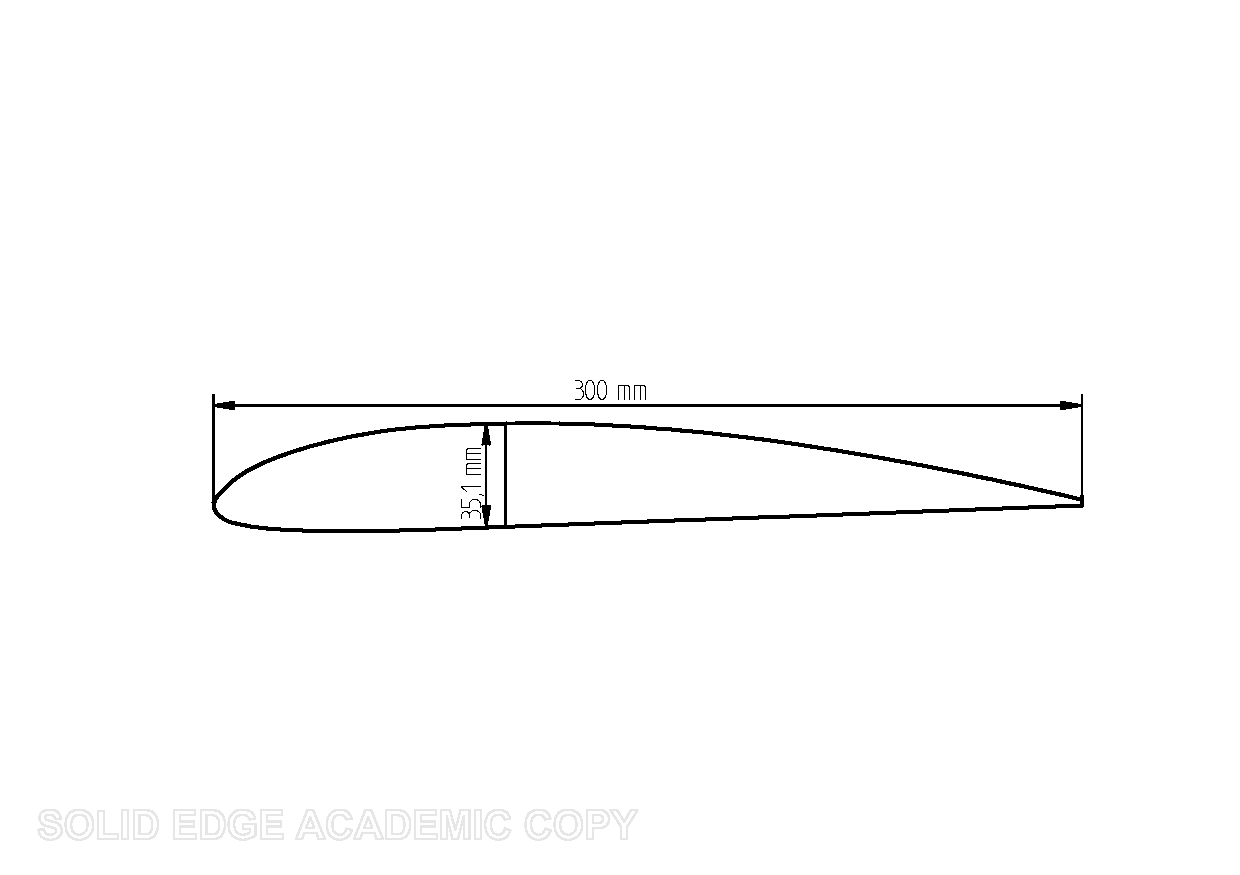
\includegraphics[width=0.9\textwidth, trim={15mm 40mm 15mm 40mm},clip]{bilder/Fotos/Tragflaechensegment.pdf}
\caption{Querschnitt durch das Flügelprofil} 
\label{fig:Querschnitt durch das Flügelprofil}
\end{figure}
Die Größte zur Verfügung stehende Dicke des Profils liegt bei 28\% seiner Tiefe.

In diesem Querschnitt soll einer der Querschnitte aus \ref{fig:Mögliche Holmprofile} eingebracht werden.

\begin{figure}[H]
\centering
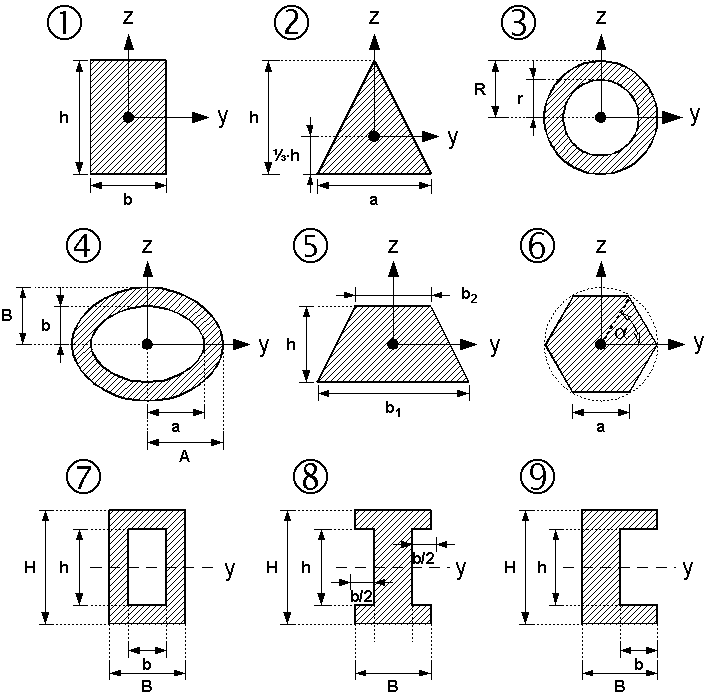
\includegraphics[width=0.9\textwidth]{bilder/Fotos/Flaechentraegheitsmoment2.png}
\caption{Mögliche Holmprofile} 
\label{fig:Mögliche Holmprofile}
\end{figure}

Für die Festigkeitsauslegung wird nach \ref{} ein Sicherheitsfaktor von $ J = 1,5 $ gewählt. Die Materialwerte werden nach \ref{Materialwerte} betrachtet.

\section{Nötiger Fertigungsaufwand}

Zur Herstellung der Verschiedenen Bauweise ist ein zum Teil erheblich unterschiedlicher Produktionsaufwand von nöten. Insbesondere die Herstellung von Vorrichtungen und Formen unterscheidet sich zwischen den Methoden. 